%%%%%%%%%%%%%%%%%%%%%%%%%%%%%%%%%%%%%%%%%%%%%%%%%%%%%%%%%%%%%%%%%%%%%%%%
% Golden Sacra - Memoria
% Escuela Politécnica Superior de la Universidad de Alicante
% Realizado por: Ángel Jesús Terol Martínez
% Contacto: jtm37@alu.ua.es
%%%%%%%%%%%%%%%%%%%%%%%%%%%%%%%%%%%%%%%%%%%%%%%%%%%%%%%%%%%%%%%%%%%%%%%%

\chapter{Estado del Arte}
\label{gb}

\section{Game Boy}
La \textbf{Game Boy} es una video consola portátil de \textbf{8 bits} desarrollada y manufacturada por Nintendo. Es la segunda consola portátil de la compañía siguiendo a su familia antecesora \textit{Game \& Watch}, saliendo al mercado el \textbf{21 de Abril de 1989 en Japón}, 3 meses más tarde en América y el 28 de Septiembre de 1990 en Europa. \\

\begin{figure}[h]
\centering
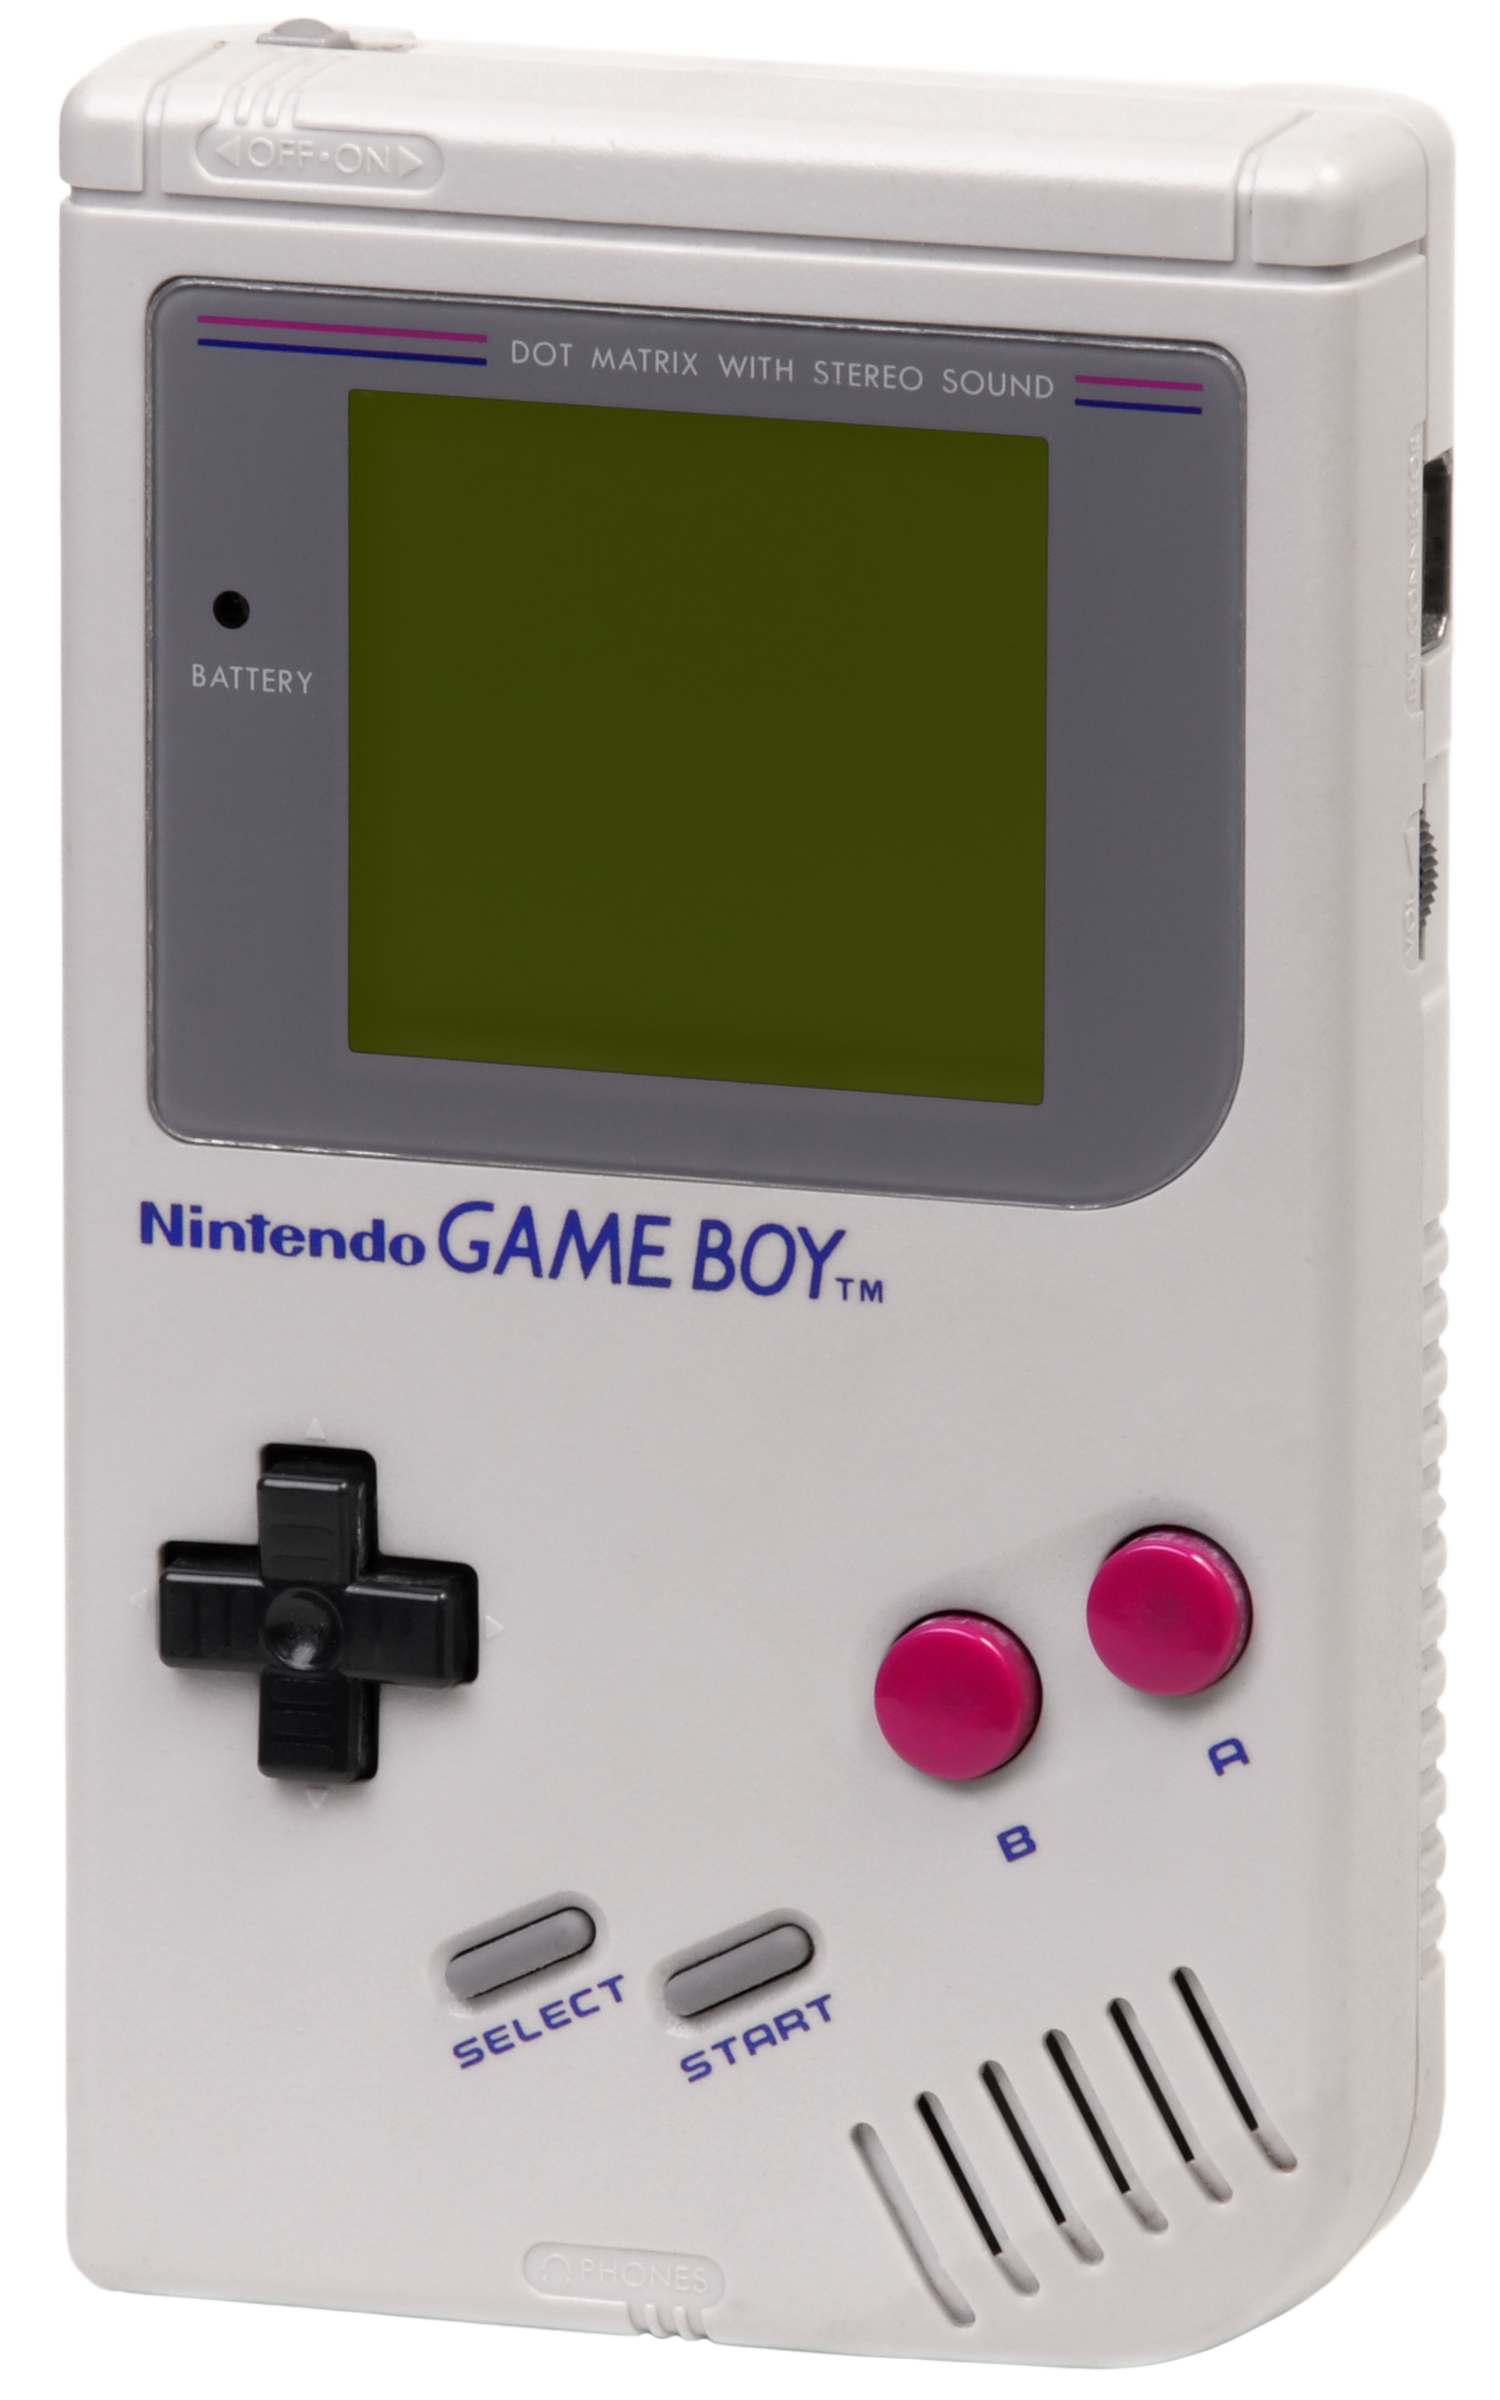
\includegraphics[width=0.15\textwidth]{include/images/GameBoy/Game-Boy-Original.jpg}
\caption{Game Boy}
\label{figure:mt_gameboy}
\end{figure}

Se caracteriza por constar de un \textbf{procesador Z80}, una \textbf{pantalla LCD} monocroma con contraste ajustable, un \textbf{pad de 8 direcciones}, \textbf{dos botones de acción} (A y B), y \textbf{dos botones de control} (Start y Select). \\ \\
Fue \textbf{duramente criticada} por diversas compañías debido al \textbf{tamaño de su pantalla y sus dos únicos colores}. Pese a ello, el hecho de que solamente se necesitasen \textbf{cuatro pilas AA} y pudieses \textbf{jugar durante días sin tener que cambiarlas} fue lo que propició su rotundo \textbf{éxito} frente a consolas como la \textit{Game Gear} de SEGA. A ello se sumó que la consola saliese a la venta en pack junto al aclamado título \textbf{Tetris}. \textbf{Tanto niños como adultos} quisieron hacerse con su propia Game Boy. \\

Por último, mencionar que si la Game Boy tuvo \textbf{tantos años de vida} fue gracias al \textbf{modelo de negocio} que aún mantiene hoy en día Nintendo, sacando \textbf{revisiones} de esta misma, \textbf{retrocompatibles} las unas con las otras, en vez de consolas completamente nuevas. Dichas consolas fueron las siguientes: \textbf{Game Boy Pocket} en 1996, y tanto \textbf{Game Boy Light} como \textbf{Game Boy Color} en 1998.

\subsection{Especificaciones Técnicas}

Cuando uno piensa en programar para cierta máquina lo primero que debe hacer es conocer exactamente \textbf{cómo es por dentro y cómo funciona}. En la siguiente tabla quedan reflejadas todas las \textbf{características de la Game Boy original}:

\begin{table}[h!]
\centering
\begin{tabular}{ |p{3.5cm}|p{3.5cm}| }

\hline

\multicolumn{2}{|c|}{\textbf{Game Boy}}             \\ \hline
CPU                & Sharp LR35902, 8-bit           \\ \hline
RAM                & 8 Kb                           \\ \hline
VRAM               & 8 Kb                           \\ \hline
Velocidad de Reloj & 4,19 MHz                       \\ \hline
OAM                & 160 bytes                      \\ \hline
Pantalla           & LCD, 2,6''                     \\ \hline
Resolución         & 160 x 144 pixeles              \\ \hline
Alimentación       & 4 pilas AA                     \\ \hline
Sonido             & 4 canales estéreo              \\ \hline
Paleta de colores  & 2-bit (4 tonos de gris)        \\ \hline
\end{tabular}

\caption{Especificaciones técnicas de la Game Boy original}

\label{table:1}
\end{table}

Estas son las \textbf{características que más nos interesan} a la hora de programar en la consola. Puede que ahora mismo te parezcan \textbf{datos sin ningún valor}, pero más tarde nos servirán de guía para conocer de \textbf{cuánta memoria disponemos en cada momento y qué podemos o no hacer}.

\clearpage

\section{Análisis del Mercado}

Si pudiésemos viajar atrás en el tiempo (unos 20 años aproximadamente), comprobaríamos cómo la GB fue una de las consolas con \textbf{mayor auge en ventas de la historia}.
\\ \\
Lamentablemente, en la actualidad, la consola ha pasado a mejor vida. En donde antes se necesitaba de un cartucho del tamaño de la palma de mi mano, ahora es posible \textbf{almacenarlos en masa} en una misma micro SD. Las personas a las que les gustan estos juegos no se van a pensar dos veces el \textbf{descargar un emulador} para su teléfono móvil, donde pueden jugarlos sin ningún tapujo.
\\ \\
Sin embargo, existe el \textbf{mercado al por menor}, donde algunas personas siguen buscando juegos originales por puro \textbf{coleccionismo}, o las \textit{scenes}, donde la gente saca diferentes demos o prototipos con los que probar los límites de la consola o simplemente pasar un buen rato.

\section{Principales Referentes}

En esta sección se encuentran todas aquellas entregas que, tras una revisión de los mismos, se cree que \textbf{han sido de utilidad} por su parecido a la hora de desarrollar este proyecto:

\subsection{Pokémon Rojo/Azul - Game Boy}

Juegos RPG conocidos en Japón como \textit{Pocket Monsters: Aka \& Midori}, desarrollados por la compañía \textbf{Game Freak} y publicados por \textbf{Nintendo}.
\\ \\
Son las \textbf{primeras entregas} de la conocida saga, siendo lanzados al mercado entre los años 1996 y 1999.

\begin{figure}[h]
\centering
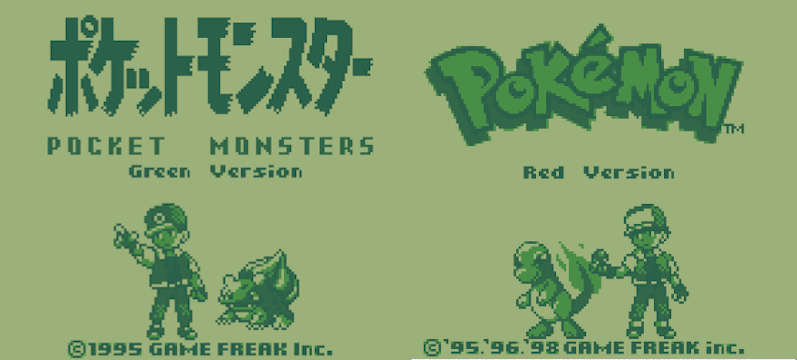
\includegraphics[width=0.6\textwidth]{include/images/GameBoy/pokemon.png}
\caption{Pokemon Azul/Rojo}
\label{figure:poke_rb}
\end{figure}

En el juego, el personaje es manejado desde una \textbf{perspectiva aérea}. El objetivo principal es llegar a conseguir/coleccionar todos los monstruos (conocidos como \textit{pokémons}) que aparecen en las distintas áreas de la región ficticia de \textit{Kanto}. Con ellos podrás completar una enciclopedia interna del juego llamada \textit{Pokédex}, la cual dispone información de las 151 especies. Todas las versiones se componen del mismo argumento y son independientes la una de la otra, pero es necesario hacer intercambios (mediante el \textit{Game Link Cable\footnote{También conocido como \textbf{Cable Link}, es un accesorio que permite conectar más de una Game Boy entre sí para jugar en modo multijugador.}}) con otros amigos para poder completarla.
\\ \\
Por otro lado, el segundo objetivo principal es que el jugador se convierta en el \textbf{entrenador pokémon} más fuerte de la región, teniendo que derrotar a todos los NPC's\footnote{NPC o \textit{Non Playable Character}, hace referencia a todos aquellos personajes que el jugador no puede controlar.} (o al menos a la mayor parte) que se lleguen a interponer por su camino.
\\ \\
Todo consta de \textbf{tres pantallas de juego} diferentes: el \textbf{mapa general}, donde el jugador maneja al protagonista desde la perspectiva aérea ya mencionada, una \textbf{pantalla de batalla} con vista lateral, donde solamente se ve nuestro \textit{pokémon} y el del rival, y la \textbf{interfaz gráfica/sistema de menús} donde se podrán configurar los \textit{pokémons} que tengamos en el equipo.

\begin{figure}[h]
\centering
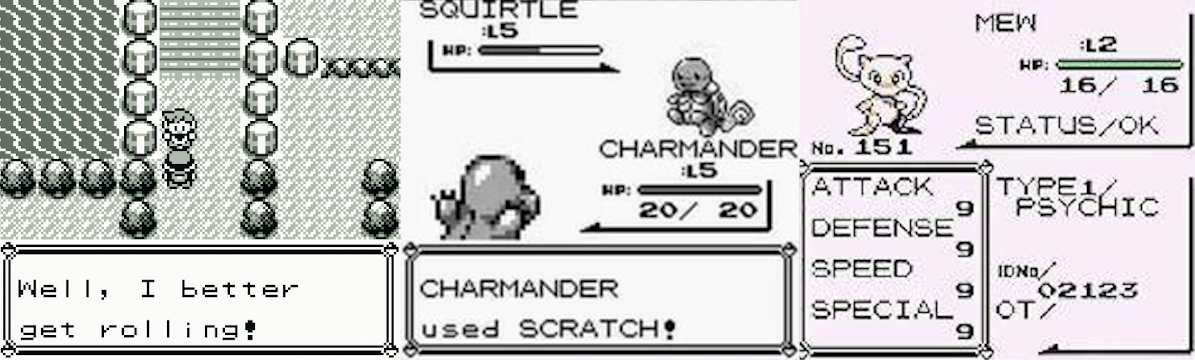
\includegraphics[width=1\textwidth]{include/images/GameBoy/pokemon_screens.png}
\caption{Pantallas de Pokémon Rojo/Azul}
\label{figure:poke_rb_screens}
\end{figure}

La \textbf{razón de escoger este título} como referente se debe a la manera en la que implementa distintos aspectos, ya sea al \textbf{renderizado de la interfaz gráfica}, el \textbf{muestreo de diálogos}, la recolección de objetos esparcidos por el mapa, o incluso el método de carga de mapas de fondo.
\\ \\
La manera en que implementa las colisiones del jugador con el mapa de fondo se van intentar replicar respecto a la forma en que este lo hace. Básicamente disponemos de distintas casillas (el jugador siempre tiene guardado su casilla actual), las cuales poseen un valor que nos indicará si se trata de una obstáculo o no.
\\ \\
También tiene implementado en su código (siendo una de las pocas entregas que lo tienen) el cambio de paletas de color. Este es un aspecto muy interesante ya que le hacía cobrar vida en la Game Boy Color. Lo veremos en el capítulo de \textbf{Desarrollo} del documento.
\\ \\
Además, de forma subjetiva, el \textbf{estilo artístico} llevado a cabo es uno de mis favoritos. Esto hará que, de forma inconsciente, la mayor parte de mis sprites estén inspirados en los suyos y pueda apreciarse a simple vista.

\subsubsection{Dibujado de Ventanas Emergentes en Pokémon Rojo/Azul}

Un análisis que se ha hecho de estas entregas es del \textbf{cómo eran capaces de dibujar múltiples ventanas} emergentes, sin necesidad de apagar la pantalla LCD.

\begin{figure}[h]
\centering
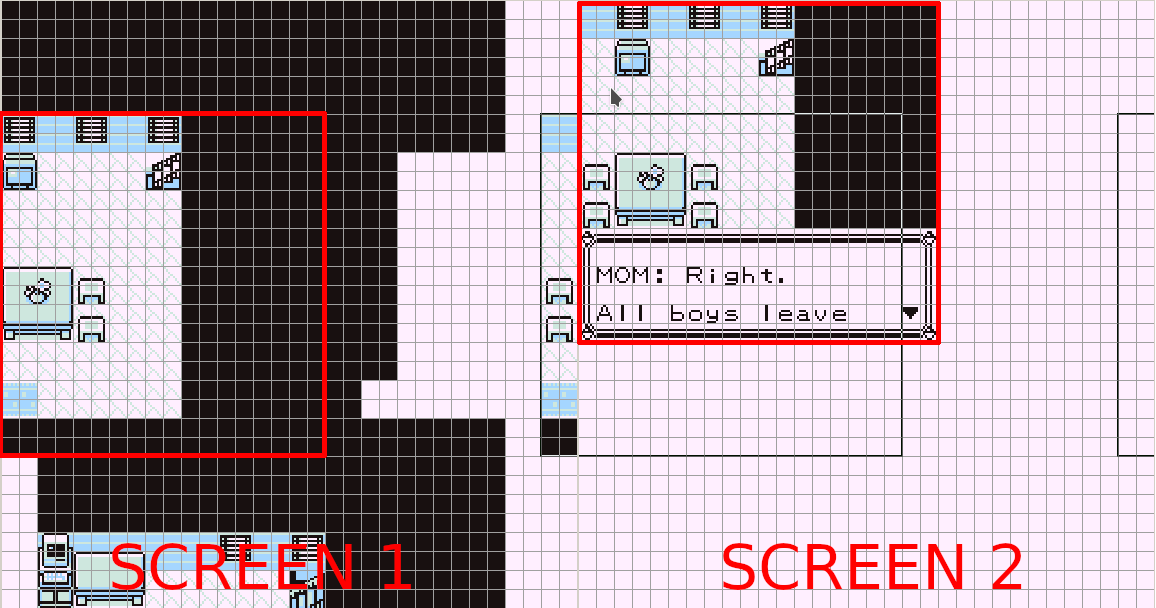
\includegraphics[width=0.6\textwidth]{include/images/desarrollo/screensdialog.png}
\caption{Dibujado de Ventanas en Pokémon Rojo/Azul}
\label{figure:drawtextspoke}
\end{figure}

Como podéis observar en las imágenes, por un lado tenemos la \textbf{pantalla principal} donde el tilemap está cargado y en la segunda, lo que nos encontramos curiosamente, es un \textbf{copiado y pegado} de todos los tiles de fondo que el scroll es capaz de mostrar en la primera. Con ello consiguen tener un \textbf{escena completamente idéntica}, lo que implica que, al superponer la segunda pantalla a la primera, no se va a captar diferencia alguna. La \textbf{ventaja} que tienen es la de \textbf{ser capaces de mostrar todas las ventanas emergentes que necesiten}, como se muestra en la siguiente imagen:

\begin{figure}[h]
\centering
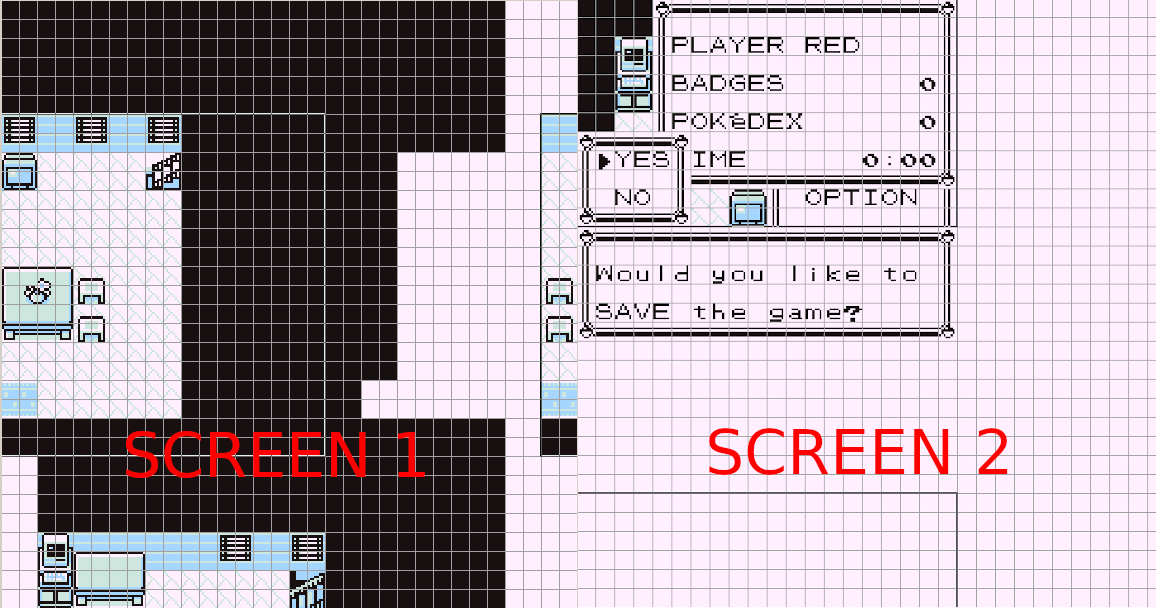
\includegraphics[width=0.6\textwidth]{include/images/desarrollo/windowspokemon.png}
\caption{Ventanas Emergentes en Pokémon Rojo/Azul}
\label{figure:windowspoke}
\end{figure}

Para conseguir crear este efecto sin necesidad de apagar la pantalla realizan lo siguiente: por cada N tiles a dibujar, \textbf{esperan previamente a un intervalo V-Blank o H-Blank} para que la memoria de vídeo no se corrompa. Además, al haber dibujado solamente en la pantalla secundaria, para volver al juego solo tienen que esconderla, sin necesidad de más.

\subsection{Pokémon Mundo Misterioso: Equipo de Rescate Rojo - Game Boy Advance}

Entrega de la saga Pokémon lanzada en el año 2006 para Europa. Existe una \textbf{versión paralela} lanzada para la consola \textbf{Nintendo DS}.

\begin{figure}[h]
\centering

\includegraphics[width=0.6\textwidth]{include/images/GameBoy/pokemon_mdr.png}
\caption{Pokemon Mundo Misterioso: Equipo de Rescate Rojo}
\label{figure:poke_mdr}
\end{figure}

Es un \textbf{RPG de aventuras} donde, a diferencia de otras entregas de la saga, innova con la premisa de que el jugador ahora es un \textit{pokémon}. El objetivo consta en rescatar al mundo de las desgracias naturales formando un equipo de rescate junto a otros \textit{pokémons}.
\\ \\
El concepto "mazmorra" ya había sido utilizada previamente en otras entregas como \textit{Shiren the Wanderer}, pero nunca en la saga \textit{Pokémon}. Todos los elementos "humanos" de otras entregas se han eliminado y ha conseguido diferenciarse de la competencia por su \textbf{argumento único y especial}.
\\ \\
La saga \textit{Mundo Misterioso} funciona mediante \textbf{turnos}. De esta manera, cada vez que el jugador se mueva, ataque, o realice cualquier otra acción, consumirá su turno, dando paso al turno de los \textit{pokémons} aliados y rivales.
\\ \\
Las \textbf{misiones se realizarán siempre en el interior de una mazmorra}, donde rescataremos \textit{pokémons} que se hayan perdido, recolectar distintos objetos importantes, o derrotar un jefe. Dichas mazmorras están \textbf{formadas por distintos pisos} a los cuales podremos acceder mediante unas escaleras que deberemos encontrar en cada uno de ellos. Los pisos se generan de \textbf{forma procedimental}, por lo que todo cambiará cada vez que entremos a la misma mazmorra, beneficiando así la rejugabilidad.

\begin{figure}[h]
\centering
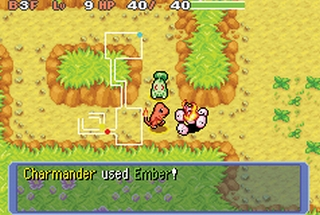
\includegraphics[width=0.6\textwidth]{include/images/GameBoy/pokemon_mdr2.png}
\caption{Captura de Pantalla In-Game de Pokémon Mundo Misterioso}
\label{figure:poke_mdr2}
\end{figure}

El juego se ha escogido como \textbf{referente} por ser exactamente el \textbf{mismo género} al cual pretendemos hacer. Las \textbf{mecánicas} van a ser \textbf{prácticamente idénticas}, con la diferencia de intentar hacerlas mucho \textbf{más simples}. Hay que tener en cuenta que este juego fue desarrollado para una consola mucho superior sobre la que vamos a trabajar.
\\ \\
La mecánica de turnos, mazmorras generadas procedimentalmente, ataques, objetos, etc..., van a estar inspiradas principalmente en esta entrega, dejando de lado temas más técnicos como los mencionados en el anterior referente.
\\ \\

\subsection{The Legend Of Zelda: Oracle of Ages - Game Boy Color}

Junto a \textit{The Legend Of Zelda: Oracle Of Seasons}, fueron dos entregas de acción/aventura desarrolladas por la compañía \textit{Flagship} y publicadas por \textit{Nintendo} para la consola Game Boy Color en el año 2001.

\begin{figure}[h]
\centering
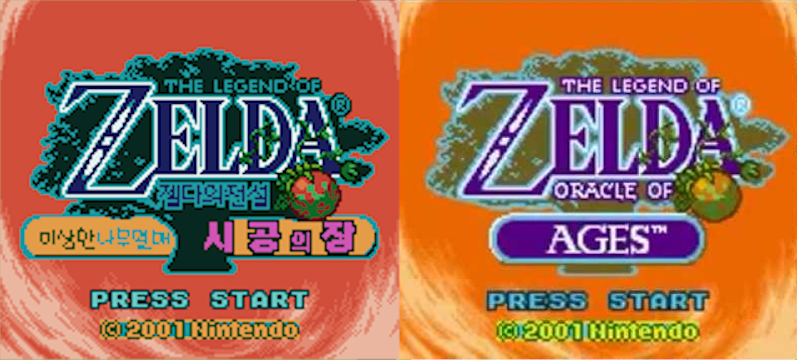
\includegraphics[width=0.8\textwidth]{include/images/GameBoy/zelda_title.png}
\caption{The Legend Of Zelda: Oracle Of Ages}
\label{figure:zelda_title}
\end{figure}

Como la mayoría de los \textit{Zelda} clásicos, el combate y la exploración se realizan desde una perspectiva aérea (similar a la de \textit{Pokémon Rojo/Azul}). El arma principal es la espada, con la que podremos golpear los enemigos en un radio determinado de distancia. También \textbf{obtendremos} a lo largo del transcurso del juego \textbf{distintos objetos que aumentarán el número de mecánicas disponibles} y ayudarán a resolver puzzles.
\\ \\
En esta entrega en particular, el protagonista deberá viajar entre el pasado y el presente, conectados por agujeros temporales, para desbloquear nuevas áreas del mapa. Esto lo podremos hacer nada más conseguir el \textit{Harpa del Tiempo} al inicio del juego.

\begin{figure}[h]
\centering
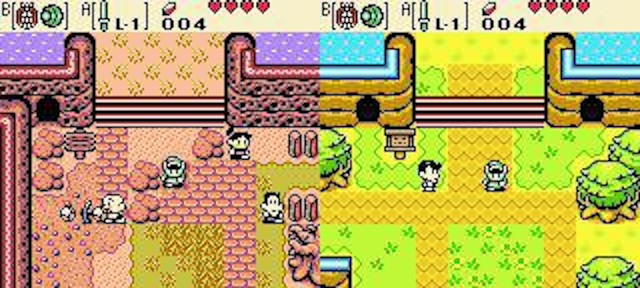
\includegraphics[width=0.6\textwidth]{include/images/GameBoy/zelda_pp.jpg}
\caption{Pasado y Presente en Oracle Of Ages}
\label{figure:zelda_pp}
\end{figure}

También encontraremos \textbf{coleccionables} que nos serán de utilidad a la hora de \textbf{mejorar el equipamiento}. En este caso, principalmente, serán anillos, que proporcionarán habilidades extras (como mejora de defensa o ataque). El poder de la espada y el escudo que el protagonista porta se podrán mejorar de forma similar hasta un máximo de dos veces.

\begin{figure}[h]
\centering
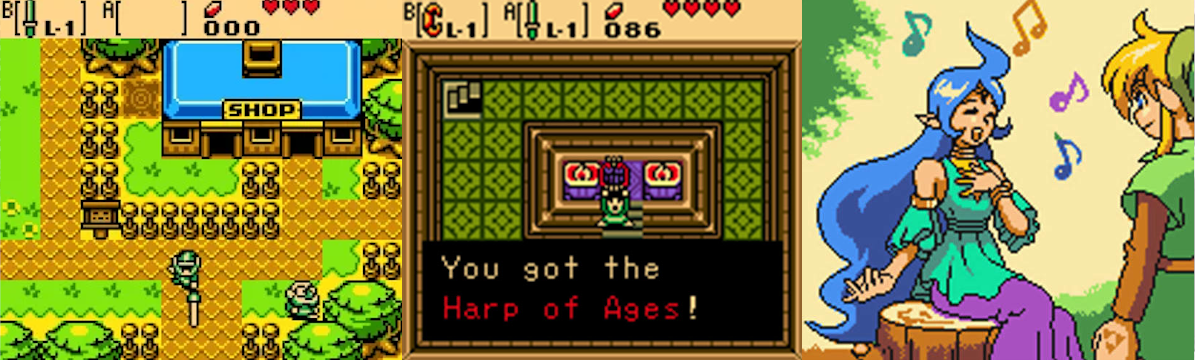
\includegraphics[width=0.8\textwidth]{include/images/GameBoy/zelda_screens.png}
\caption{Capturas de Pantalla In-Game del Oracle Of Ages}
\label{figure:zelda_screens}
\end{figure}

La entrega fue un \textbf{éxito tanto en lo que ventas se refiere como en crítica}. En la revista \textit{Nintendo Power}, fue posicionado en el número 39 de los 200 mejores juegos de la consola.
\\ \\
La razón de escoger esta entrega como referente es el \textbf{diseño artístico de sus enemigos}, cargado de mapas de fondo y movimiento del scroll (distintos a como se implementó en \textit{Pokémon}). El hecho de que puedas obtener coleccionables para futuras mejoras y el poder obtener distintas armas también es un factor que voy a tener en cuenta para mejorar la experiencia de juego.

\cleardoublepage %salta a nueva página impar




